\documentclass{article}

\usepackage[italian]{babel}
\usepackage[margin=2cm, footskip=5mm]{geometry}
% questi package non sono necessari in lualatex; ref https://tex.stackexchange.com/a/413046
% \usepackage[utf8]{inputenc}
% \usepackage[T1]{fontenc}
\usepackage{enumitem}
\usepackage{hyperref}
\usepackage{titlesec}
\usepackage{soulutf8}
\usepackage{contour}
\usepackage{float}
\usepackage{graphicx}
\usepackage{fancyhdr}
\usepackage{longtable}
\usepackage[table]{xcolor}
\usepackage{titling}
\usepackage{lastpage}
\usepackage{ifthen}
\usepackage{calc}
\usepackage{minted}
\usepackage{pgfgantt}
\usepackage{subfiles}

\newlength{\imgwidth}

\newcommand\scalegraphics[1]{%
    \settowidth{\imgwidth}{\includegraphics{#1}}%
    \setlength{\imgwidth}{\minof{\imgwidth}{\textwidth}}%
    \includegraphics[width=\imgwidth]{#1}%
}

% XXX definizione dei percorsi in cui cercare immagini
\graphicspath{ {./}
    {./img/}
}

% esempio di utilizzo: \appendToGraphicspath{./img/} (un comando diverso per ogni path da includere)
% N.B.: ci DEVE essere un forward slash alla fine del path, a indicare che è una cartella.
\makeatletter
\newcommand\appendToGraphicspath[1]{%
  \g@addto@macro\Ginput@path{{#1}}%
}
\makeatother

% setup della sottolineatura
\setuldepth{Flat}
\contourlength{0.8pt}

\newcommand{\uline}[1]{%
  \ul{{\phantom{#1}}}%
  \llap{\contour{white}{#1}}%
}

% setup dei link
\hypersetup{
  colorlinks=true, % set true if you want colored links
  linktoc=all,     % set to all if you want both sections and subsections linked
  linkcolor=black, % choose some color if you want links to stand out
}

% setup di header e footer
\pagestyle{fancy}

\fancyhf{}
\fancyhead[L]{\includegraphics[width=1cm]{logo.png}}
\fancyhead[R]{\thetitle}
\fancyfoot[R]{\thepage\ di~\pageref{LastPage}}

\fancypagestyle{nopage}{%
  \fancyfoot{}%
}

\setlength{\headheight}{1.2cm}

% setup forma \paragraph e \subparagraph
\titleformat{\paragraph}[hang]{\normalfont\normalsize\bfseries}{\theparagraph}{1em}{}
\titleformat{\subparagraph}[hang]{\normalfont\normalsize\bfseries}{\thesubparagraph}{1em}{}

% setup profondità indice di default
\setcounter{secnumdepth}{5}
\setcounter{tocdepth}{5}

% shortcut per i placeholder
\newcommand{\plchold}[1]{\textit{\{#1\}}} % chktex 20

% hook per lo script che genera il glossario
\newcommand{\glossario}[1]{\underline{#1}\textsubscript{g}}

% definizione dei comandi \uso e \stato
\makeatletter
\newcommand{\setUso}[1]{%
  \newcommand{\@uso}{#1}%
}
\newcommand{\uso}{\@uso}

\newcommand{\setStato}[1]{%
  \newcommand{\@stato}{#1}%
}
\newcommand{\stato}{\@stato}

\newcommand{\setVersione}[1]{%
  \newcommand{\@versione}{#1}%
}
\newcommand{\versione}{\@versione}

\newcommand{\setResponsabile}[1]{%
  \newcommand{\@responsabile}{#1}%
}
\newcommand{\responsabile}{\@responsabile}

\newcommand{\setRedattori}[1]{%
  \newcommand{\@redattori}{#1}%
}
\newcommand{\redattori}{\@redattori}

\newcommand{\setVerificatori}[1]{%
  \newcommand{\@verificatori}{#1}%
}
\newcommand{\verificatori}{\@verificatori}

\newcommand{\setDescrizione}[1]{%
  \newcommand{\@descrizione}{#1}%
}
\newcommand{\descrizione}{\@descrizione}

\newcommand{\setModifiche}[1]{%
  \newcommand{\@modifiche}{#1}%
}

\newcommand{\modifiche}{\@modifiche}

\makeatother

% setup delle description
\setlist[description,1]{font=$\bullet$\hspace{1.5mm}, labelwidth=* leftmargin=*,labelindent=12.5mm}
\setlist[description,2]{font=$\bullet$\hspace{1.5mm}, leftmargin=*,labelindent=12.5mm}
\appendToGraphicspath{../../commons/img/}

\title{Verbale interno --- 25/02/2020}

\setResponsabile{Alessandro Rizzo}
\setRedattori{Alessandro Rizzo}
\setVerificatori{
  Alberto Cocco
}
\setUso{Interno}
\setDescrizione{Verbale dell'incontro di GruppOne del 25/02/2020}
\setModifiche{%
\cellcolor{white!80!lightgray!100}& Alessandro Rizzo & 2020--02--27 & approva documento \\%
\cellcolor{white!80!lightgray!100}& Alberto Cocco & 2020--02--26 & verifica verbale \\%
\multirow{-3}{*}{0.1.0}& Alessandro Rizzo & 2020--02--25 & stendi verbale %
}

\begin{document}

\thispagestyle{empty}
\pagenumbering{gobble}

\begin{center}

  \includegraphics[width=8.5cm]{\commons/img/logo.png}\\
  {\Large GruppOne - progetto "Stalker"}\\
  \vspace{1.5cm}

  {\Huge \thetitle}
  \vspace{1.5cm}

  \begin{table}[H]
    \centering

    \begin{tabular}{r|l}
      \textbf{Versione}     & \versione              \\
      \textbf{Approvazione} & \responsabile          \\
      \textbf{Redazione}    & \redattori             \\
      \textbf{Verifica}     & \verificatori          \\
      \textbf{Stato}        & \stato                 \\
      \textbf{Uso}          & \uso                   \\
      \textbf{Destinato a}  & Imola Informatica      \\
                            & GruppOne               \\
                            & Prof. Tullio Vardanega \\
                            & Prof. Riccardo Cardin  \\
    \end{tabular}
  \end{table}

  \vspace{3cm}
  \textbf{Descrizione}\\
  \descrizione\\
  \vfill
  \verb|gruppone.swe@gmail.com|
\end{center}

\newpage
\thispagestyle{nopage}

\section*{Registro delle modifiche}
\label{sec:registro_delle_modifiche}

\begin{table}[H]
  \label{tab:registro_delle_modifiche}

  \centering
  \rowcolors{2}{lightgray}{white!80!lightgray!100}

  \begin{longtable}[c]{c c c c l}
    \rowcolor{darkgray!90!}\color{white}{\textbf{Versione}} & \color{white}{\textbf{Data}} & \color{white}{\textbf{Nominativo}} & \color{white}{\textbf{Ruolo}} & \color{white}{\textbf{Descrizione}} \\\endhead
    \modifiche
  \end{longtable}
\end{table}

% section registro_delle_modifiche (end)
\newpage

\thispagestyle{nopage}
\pagenumbering{roman}
\tableofcontents

\newpage

\pagenumbering{arabic}


\section{Informazioni logistiche}%
\label{sec:informazioni_logistiche}

\begin{description}
  \item [Luogo] chiamata Hangouts
  \item [Data] 25/02/2020
  \item [Ora] 13:00 \symbol{8594} 14:00
\end{description}

\subsection{Membri del gruppo presenti}%
\label{sub:membri_del_gruppo_presenti}

\begin{enumerate}
  \item Riccardo Agatea
  \item Alberto Cocco
  \item Luca Ercole
  \item Alberto Gobbo
  \item Alessandro Rizzo
  \item Fabio Scettro
\end{enumerate}
% sub:membri_del_gruppo_presenti (end)
% sec:informazioni_logistiche (end)

\section{Introduzione}%
\label{sec:introduzione}

Abbiamo discusso delle tecnologie del PoC per allinearci e stabilire i compiti per i giorni a seguire, inoltre ci siamo confrontati sul registro delle modifiche per raggiungere un sistema di versionamento più comprensibile.

\section{Ordine del giorno}%
\label{sec:ordine_del_giorno}

\begin{itemize}
  \item Discussione sulle tecnologie PoC
  \item Registro delle modifiche.
\end{itemize}
% sec:ordine_del_giorno (end)
\section{Discussione sulle Tecnologie del PoC}%
\label{sec:discussione_tecnologie_poc}
I membri del gruppo hanno discusso le tecnologie apprese per ora singolarmente per scegliere quelle più idonee al progetto.
Per la web-app e l'applicazione mobile sono emersi i framework \glossario{Nativescript} e \glossario{Angular} che insieme permettono di riutilizzare buona parte del codice tra le due interfacce, per la geolocalizzazione mobile l'opzione migliore sembrano essere i servizi di \glossario{geofencing} offerti da Google mentre per selezionare posizioni sulle mappe l'opzione dominante è \glossario{OpenStreetMap}
Per quanto riguarda il server le tecnologie più interessanti sono \glossario{Kubernetes} per la gestione della scalabilità del server, mentre per implementare il server si pensava a due layer, uno per accogliere dati permanenti come utenti e organizzazioni e uno per contenere dati più leggeri e non permanenti nel tempo come le posizioni degli utenti.
Per il primo tipo di dati verrà usato un database MySQL mentre per il secondo verrà utilizzato un database time series, specializzato in gestire grandi flussi di dati di questo tipo.
La linea guida per ora è raccogliere tutte le chiamate di rete possibili tra server e applicazione in una API che rispetta la specifica REST utilizzando \glossario{Swagger} e continuare ad approfondire le tecnologie che sono risultate più convincenti.
% sec:discussione_tecnologie_poc (end)

\section{Registro delle modifiche}%
\label{sec:registro_modifiche}
L'elemento che generava confusione nel registro delle modifiche era la presenza ripetuta dello stesso numero di versione in più righe diverse e lo scatto di versione solamente all'approvazione del documento, così facendo si perdeva la correlazione tra azione e approvazione.
Abbiamo quindi deciso di associare un unico numero all'intero processo di azione, verifica e approvazione che consisterà in un unica versione.
% sec:registro_modifiche (end)

\newpage
\section{Registro delle decisioni}%
\label{sec:registro_delle_decisioni}

\begin{table}[H]
  \centering
  \rowcolors{2}{lightgray}{white!80!lightgray!100}
  \renewcommand{\arraystretch}{2}
  \begin{tabular}{c b{13cm}}
    \rowcolor{darkgray!90!}\color{white}{\textbf{Codice}} & \color{white}{\textbf{Decisione}}\\
    1 & Abbiamo deciso di iniziare a scrivere le chiamate di rete per andare a definire una API REST da cui poi sviluppare il nostro PoC.\\
    2 & Modificheremo il registro delle modifiche come sopra per riflettere azione, verifica e approvazione come parti di una unica versione che si concretizza al momento della approvazione delle modifiche.\\
  \end{tabular}
  \caption{registro delle decisioni}%
  \label{tab:registro delle decisioni}
\end{table}
% sec:registro_delle_decisioni (end)

\end{document}
